\sect{Hybrid Basis and Coordinate Calculus}\label{sec:hybridCalculus}

% Motivation: Effective Coordinate Calculus
In some situations, we can perform basis calculus more effectively by avoiding image enumeration variables, and instead apply coordinatewise transforms on tensors (see \defref{def:coordinatewiseTransform}).
As we show here, these include conjunctions, which correspond with coordinatewise multiplication, and negation, which correspond with coordinatewise subtraction from the trivial tensor.
Such schemes are applied for example in \cite{tsilionis_tensor-based_2024} in batchwise logical inference.

\begin{figure}
    \begin{center}
        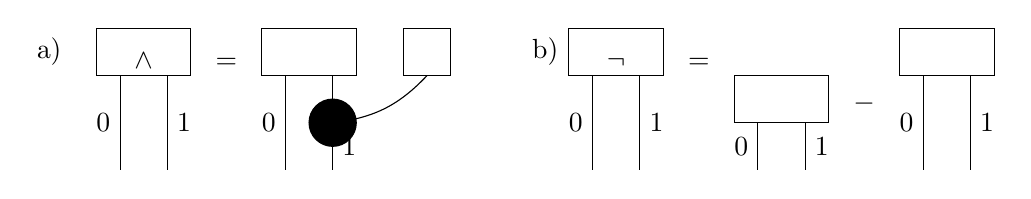
\begin{tikzpicture}[scale=0.3] 

\node at (-12,2) [above]  {a)};

	\begin{scope}[shift={(-7,0)}]
	  	\draw[]  (-3,2) rectangle (1,4);
		\node at (-1,1.9) [above] {${\exformula\land\secexformula}$};
		\draw (-2,2) -- (-2,-2) node[midway,left] {$\catvariableof{0}$};
		\draw (0,2) -- (0,-2) node[midway,right] {$\catvariableof{1}$};	
	\end{scope}
	\node at (-4.5,1.9) [above] {$=$};	
  	\draw[] (-3,2) rectangle (1,4);
	\node at (-1,1.9) [above] {${\exformula}$};
  	\draw[] (3,2) rectangle (5,4);
	\node at (4,1.9) [above] {${\secexformula}$};
	
	\node at (0,0) [left,] {$\delta$};
	\draw[]  (0,2) -- (0,0);% node[midway,left] {$\placeholderof{1}$};
	\draw[fill,] (0,0) circle (\dotsize);
	\draw[] (0,0) -- (0,-2) node[midway,right] {$\catvariableof{1}$};
	\draw[] (4,2) to[bend left=20] (0,0);
	\draw[] (-2,2) -- (-2,-2) node[midway,left] {$\catvariableof{0}$};

\begin{scope}[shift={(27,0)}]
	\node at (-18,2) [above]  {b)};
  	\begin{scope}[shift={(-14,0)}]
	  	\draw[]  (-3,2) rectangle (1,4);
		\node at (-1,1.9) [above] {${\lnot\exformula}$};
		\draw (-2,2) -- (-2,-2) node[midway,left] {$\catvariableof{0}$};
		\draw (0,2) -- (0,-2) node[midway,right] {$\catvariableof{1}$};	
	\end{scope}
	
    	\begin{scope}[shift={(-2,-2)}]
  		\draw[] (-8,2) rectangle (-4,4);
		\node at (-6,2) [above,] {$\ones$};
		\draw[] (-7,2) -- (-7,0) node[midway,left] {$\catvariableof{0}$};
		\draw[] (-5,2) -- (-5,0) node[midway,right] {$\catvariableof{1}$};
	\end{scope}
	
	\draw[] (-2,2) -- (-2,-2) node[midway,left] {$\catvariableof{0}$};
	\draw[](0,2) -- (0,-2) node[midway,right] {$\catvariableof{1}$};
	\node[] at (-4.5,0) [above] {$-$};



	\node at (-11.5,1.9) [above] {$=$};	
	
  	\draw[]  (-3,2) rectangle (1,4);
	\node at (-1,1.9) [above] {${\exformula}$};	
	
\end{scope}

\end{tikzpicture}
    \end{center}
    \caption{Decomposition schemes by hybrid calculus, using coordinatewise transforms of tensors (see \defref{def:coordinatewiseTransform}).
    a) Conjunction performed by coordinatewise multiplications.
    b) Negations performed by coordinatewise subtraction from one.}\label{fig:ConNegDecomposition}
\end{figure}

\begin{theorem}
    \label{the:effectiveConjunction}
    For any formulas $\exformula,\secexformula$ we have
    \begin{align*}
        \contractionof{
            \bencodingofat{\land}{\headvariableof{\exformula\land\secexformula},\formulavar,\secexformulavar},\tbasisat{\headvariableof{\exformula\land\secexformula}}
        }{\formulavar,\secexformulavar}
        = \tbasisat{\formulavar} \otimes \tbasisat{\secexformulavar} \, .
    \end{align*}
    In particular, it holds that (see \figref{fig:ConNegDecomposition}a)
    \begin{align*}
    (\exformula\land\secexformula)[\shortcatvariables]
        = \contractionof{\exformula,\secexformula}{\shortcatvariables} \, .
    \end{align*}
\end{theorem}
\begin{proof}
    We decompose
    \begin{align*}
        \bencodingofat{\land}{\headvariableof{\exformula\land\secexformula},\formulavar,\secexformulavar}
        = \tbasisat{\headvariableof{\exformula\land\secexformula}} \otimes \tbasisat{\formulavar} \otimes \tbasisat{\secexformulavar}
        + \fbasisat{\headvariableof{\exformula\land\secexformula}} \left( \onesat{\formulavar,\secexformulavar} -  \tbasisat{\formulavar} \otimes \tbasisat{\secexformulavar} \right)
    \end{align*}
    and get the first claim as
    \begin{align*}
        \contractionof{
            \bencodingofat{\land}{\headvariableof{\exformula\land\secexformula},\formulavar,\secexformulavar},\tbasisat{\headvariableof{\exformula\land\secexformula}}
        }{\formulavar,\secexformulavar}
        & = \contractionof{
            \tbasisat{\headvariableof{\exformula\land\secexformula}} \otimes \tbasisat{\formulavar} \otimes \tbasisat{\secexformulavar},\tbasisat{\headvariableof{\exformula\land\secexformula}}
        }{\formulavar,\secexformulavar} \\
        & = \tbasisat{\formulavar} \otimes \tbasisat{\secexformulavar} \, .
    \end{align*}
    To show the second claim we use
    \begin{align*}
    (\exformula\land\secexformula)[\shortcatvariables]
        &= \contractionof{
            \bencodingofat{\exformula}{\formulavar,\shortcatvariables},
            \bencodingofat{\secexformula}{\secexformulavar,\shortcatvariables},
            \bencodingofat{\land}{\headvariableof{\exformula\land\secexformula},\formulavar,\secexformulavar},
            \tbasisat{\headvariableof{\exformula\land\secexformula}}
        }{\shortcatvariables} \\
        &  = \contractionof{
            \bencodingofat{\exformula}{\formulavar,\shortcatvariables},
            \bencodingofat{\secexformula}{\secexformulavar,\shortcatvariables},
            (\tbasisat{\formulavar}\otimes \tbasisat{\secexformulavar})
        %\bencodingofat{\land}{\formulavar,\secexformulavar,\headvariableof{\exformula\land\secexformula}}
        }{\shortcatvariables} \\
        &= \contractionof{\exformula,\secexformula}{\shortcatvariables} \, . \qedhere
    \end{align*}
\end{proof}

A similar decomposition holds for negations, as we show next.

\begin{theorem}
    For any formula $\exformula$ we have
    \begin{align*}
        \contractionof{
            \bencodingofat{\lnot}{\headvariableof{\lnot\exformula},\formulavar},\tbasisat{\headvariableof{\lnot\exformula}}
        }{\formulavar}
        = \fbasisat{\formulavar} =  \onesat{\formulavar} - \tbasisat{\formulavar} \, .
    \end{align*}
    and
    \begin{align*}
        \contractionof{
            \bencodingofat{\lnot}{\formulavar,\headvariableof{\lnot\exformula}},\fbasisat{\headvariableof{\lnot\exformula}}
        }{\formulavar}
        = \tbasisat{\formulavar} \, .
    \end{align*}
    In particular, it holds that (see \figref{fig:ConNegDecomposition}b)
    \begin{align*}
    (\lnot\exformula)[\shortcatvariables]
        = \onesat{\shortcatvariables} - \formulaat{\shortcatvariables}  \, .
    \end{align*}
\end{theorem}
\begin{proof}
    We have
    \begin{align*}
        \bencodingofat{\lnot}{\headvariableof{\lnot\exformula},\formulavar}
        = \tbasisat{\headvariableof{\lnot\exformula}} \otimes \fbasisat{\formulavar}
        +\fbasisat{\headvariableof{\lnot\exformula}} \otimes \tbasisat{\formulavar}
    \end{align*}
    and therefore get the second claim by contraction with $\fbasisat{\headvariableof{\lnot\exformula}}$
    \begin{align*}
        \contractionof{
            \bencodingofat{\lnot}{\formulavar,\headvariableof{\lnot\exformula}},\fbasisat{\headvariableof{\lnot\exformula}}
        }{\formulavar}
        &=  \contractionof{
            \tbasisat{\headvariableof{\lnot\exformula}} \otimes \fbasisat{\formulavar},\fbasisat{\headvariableof{\lnot\exformula}}
        }{\formulavar} \\
        &\quad +  \contractionof{
            \fbasisat{\headvariableof{\lnot\exformula}} \otimes \tbasisat{\formulavar},\fbasisat{\headvariableof{\lnot\exformula}}
        }{\formulavar}
        \\
        &= \tbasisat{\formulavar} \, .
    \end{align*}
    The first equation of the first claim follows similarly by contraction with $\tbasisat{\headvariableof{\lnot\exformula}}$ as
    \begin{align*}
        \contractionof{
            \bencodingofat{\lnot}{\headvariableof{\lnot\exformula},\formulavar},\tbasisat{\headvariableof{\lnot\exformula}}
        }{\formulavar}
        = \fbasisat{\formulavar}
    \end{align*}
    and the second equation using that $\onesat{\catvariable}=\fbasisat{\catvariable}+\tbasisat{\catvariable}$ and hence
    \begin{align*}
        \fbasisat{\formulavar} =  \onesat{\formulavar} - \tbasisat{\formulavar} \, .
    \end{align*}
    To show the third claim, we contract the computation tensor $\bencodingofat{\exformula}{\formulavar,\shortcatvariables}$ to the formula $\exformula$ on both sides of the first claim and get
    \begin{align*}
        &\contractionof{
            \bencodingofat{\exformula}{\formulavar,\shortcatvariables},\bencodingofat{\lnot}{\headvariableof{\lnot\exformula},\formulavar},\tbasisat{\headvariableof{\lnot\exformula}}
        }{\formulavar} \\
        &\quad=
        \contractionof{\bencodingofat{\exformula}{\formulavar,\shortcatvariables},\onesat{\formulavar}}{\formulavar}
        - \contractionof{\bencodingofat{\exformula}{\formulavar,\shortcatvariables},\tbasisat{\formulavar}}{\formulavar} \, .
    \end{align*}
    We simplify this equation using the trivial head contraction identity of directed tensors of \corref{cor:onesHead} stating that % and \lemref{lem:formulaEncodingDecomposition}
%    For any formula $\formulaat{\shortcatvariables}$ we further have by \lemref{lem:formulaEncodingDecomposition}
    \begin{align*}
        \formulaat{\shortcatvariables} = \contractionof{\bencodingofat{\exformula}{\formulavar,\shortcatvariables},\tbasisat{\formulavar}}{\shortcatvariables}
        \andspace
        \lnot\formulaat{\shortcatvariables} = \contractionof{\bencodingofat{\exformula}{\formulavar,\shortcatvariables},\fbasisat{\formulavar}}{\shortcatvariables}
    \end{align*}
    and arrive at the third claim
    \begin{align*}
    (\lnot\exformula)[\shortcatvariables]
        = \onesat{\shortcatvariables} - \formulaat{\shortcatvariables}  \, . & \qedhere
    \end{align*}
\end{proof}

% Usage
These theorems provide a mean to represent logical formulas by sums of one-hot encodings.
Since any propositional formula can be represented by compositions of negations and conjunctions, they are universal.
We further notice, that the resulting decomposition is a basis+ CP format, as further discussed in \charef{cha:sparseRepresentation}.
In \figref{fig:DecompositionExample} we provide an example of this decomposition.


\begin{figure}
    \begin{center}
        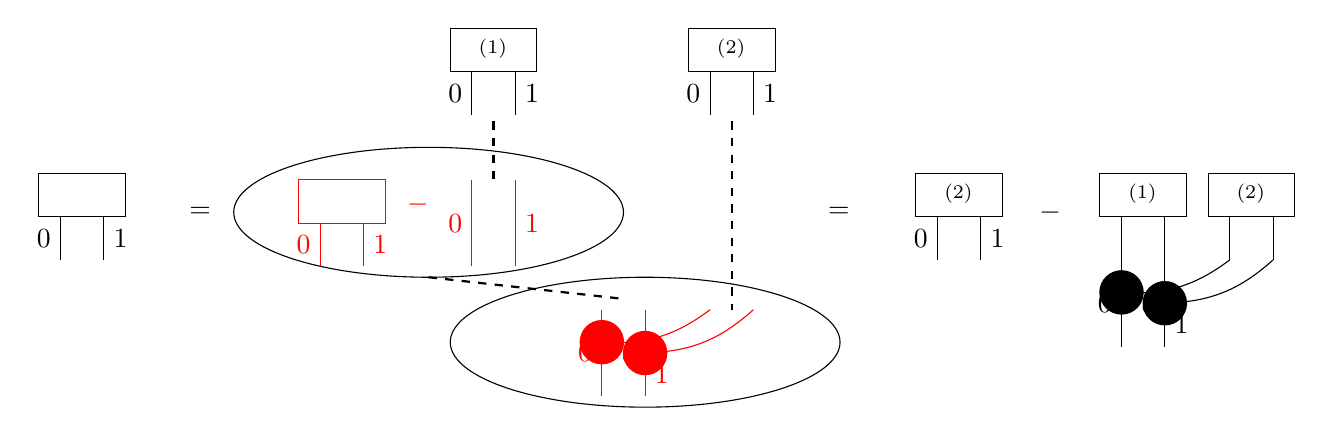
\begin{tikzpicture}[scale=0.275] % , baseline = -3.5pt



\begin{scope}[shift={(-19,-1.7)}]
		%\draw[] (-1,2.2) ellipse (4 and 2.5);
	  	\draw  (-3,2) rectangle (1,4);
		\node at (-1,1.9) [above] {${\exformula}$};
		\draw (-2,2) -- (-2,0) node[midway,left] {$\catvariableof{0}$};
		\draw (0,2) -- (0,0) node[midway,right] {$\catvariableof{1}$};	
		\node at (3.5,2.2)[right]  {$=$};
\end{scope}

\draw[] (-4,0.5) ellipse (9 and 3);
   	\begin{scope}[shift={(-2,-2)}]
  		\draw[\skeletoncolor] (-8,2) rectangle (-4,4);
		\node at (-6,2) [above,\skeletoncolor] {$\ones$};
		\draw[\skeletoncolor] (-7,2) -- (-7,0) node[midway,left] {$\catvariableof{0}$};
		\draw[\skeletoncolor] (-5,2) -- (-5,0) node[midway,right] {$\catvariableof{1}$};
	\end{scope}
	
	\draw[\skeletoncolor] (-2,2) -- (-2,-2) node[midway,left] {$\catvariableof{0}$};
	\draw[\skeletoncolor](0,2) -- (0,-2) node[midway,right] {$\catvariableof{1}$};
	\node[\skeletoncolor] at (-4.5,0) [above] {$-$};
\draw[thick,dashed] (-4,-2.5) -- (5,-3.5);
%\draw[] (6,-2.5) -- (1,-2.5);

%% Into negation core
\draw[thick,dashed] (-1,4.7) -- (-1,2);%-4,3.5);

%% Into conjunction core
\draw[thick,dashed] (10,4.7) -- (10,-4);%(6,-2.5);


\begin{scope}[shift={(10,-6)}]
	\draw[] (-4,0.5) ellipse (9 and 3);
	\begin{scope}[shift={(-4,0)}]
		\renewcommand{\skeletoncolor}{red}
	\node at (0,0) [left,\skeletoncolor] {$\delta$};
	\draw[\skeletoncolor]  (0,2) -- (0,0);% node[midway,left] {$\placeholderof{1}$};
	\draw[fill,\skeletoncolor] (0,0) circle (\dotsize);
	\draw[\skeletoncolor] (0,0) -- (0,-2) node[midway,right] {$\catvariableof{1}$};
	\draw[\skeletoncolor] (5,2) to[bend left=20] (0,0);


	\draw[fill,\skeletoncolor] (-2,0.5) circle (\dotsize);
	\draw[\skeletoncolor] (3,2) to[bend left=20] (-2,0.5);
	\draw[\skeletoncolor] (-2,2) -- (-2,-2) node[midway,left] {$\catvariableof{0}$};
	\end{scope}
\end{scope}



\begin{scope}[shift={(0,5)}]
		%\draw[] (-1,2.2) ellipse (4 and 2.5);
	  	\draw  (-3,2) rectangle (1,4);
		\node at (-1,1.9) [above] {${\secexformula^{(1)}}$};
		\draw (-2,2) -- (-2,0) node[midway,left] {$\catvariableof{0}$};
		\draw (0,2) -- (0,0) node[midway,right] {$\catvariableof{1}$};	
\end{scope}

\begin{scope}[shift={(11,5)}]
		%\draw[] (-1,2.2) ellipse (4 and 2.5);
	  	\draw  (-3,2) rectangle (1,4);
		\node at (-1,1.9) [above] {${\secexformula^{(2)}}$};
		\draw (-2,2) -- (-2,0) node[midway,left] {$\catvariableof{0}$};
		\draw (0,2) -- (0,0) node[midway,right] {$\catvariableof{1}$};	
		
\end{scope}




\node at (14,0.5)[right]  {$=$};


\begin{scope}[shift={(29,0)}]

\begin{scope}[shift={(-7.5,-1.7)}]
		%\draw[] (-1,2.2) ellipse (4 and 2.5);
	  	\draw[]  (-3,2) rectangle (1,4);
		\node at (-1,1.9) [above] {${\secexformula^{(2)}}$};
		\draw[] (-2,2) -- (-2,0) node[midway,left] {$\catvariableof{0}$};
		\draw[] (0,2) -- (0,0) node[midway,right] {$\catvariableof{1}$};	
		\node at (2.25,2.2)[right]  {$-$};		
\end{scope}


\begin{scope}[shift={(1,-3.7)}]
%	\renewcommand{\skeletoncolor}{\conjunctioncolor}
	\node at (0,0) [left] {$\delta$};
	\draw[]  (0,2) -- (0,0);% node[midway,left] {$\placeholderof{1}$};
	\draw[fill] (0,0) circle (\dotsize);
	\draw[] (0,0) -- (0,-2) node[midway,right] {$\catvariableof{1}$};
	\draw[] (5,2) to[bend left=20] (0,0);


	\draw[fill] (-2,0.5) circle (\dotsize);
	\draw[] (3,2) to[bend left=20] (-2,0.5);
	\draw[] (-2,2) -- (-2,-2) node[midway,left] {$\catvariableof{0}$};
\end{scope}


\begin{scope}[shift={(1,-1.7)}]
		%\draw[] (-1,2.2) ellipse (4 and 2.5);
	  	\draw  (-3,2) rectangle (1,4);
		\node at (-1,1.9) [above] {${\secexformula^{(1)}}$};
		\draw[] (-2,2) -- (-2,0); % node[midway,left] {$\catvariableof{0}$};
		\draw[] (0,2) -- (0,0); % node[midway,right] {$\catvariableof{1}$};	
	
\end{scope}
	
\begin{scope}[shift={(6,-1.7)}]
		%\draw[] (-1,2.2) ellipse (4 and 2.5);
	  	\draw[]  (-3,2) rectangle (1,4);
		\node at (-1,1.9) [above] {${\secexformula^{(2)}}$};
		\draw[]  (-2,2) -- (-2,0); % node[midway,left] {$\catvariableof{0}$};
		\draw[]  (0,2) -- (0,0); % node[midway,right] {$\catvariableof{1}$};	
	
\end{scope}

\end{scope}



	
	
\end{tikzpicture}
    \end{center}
    \caption{
        Example of a decomposition by hybrid calculus of a formula
        $\formulaat{\catvariableof{1},\catvariableof{2}} = \textcolor{blue}{\lnot} \secexformula^{(1)}[\catvariableof{1},\catvariableof{2}] \textcolor{red}{\land}  \secexformula^{(2)}[\catvariableof{1},\catvariableof{2}]$ into a sum of contractions.
    }\label{fig:DecompositionExample}
\end{figure}

